\documentclass[a4paper]{article}
\usepackage{polski}
\usepackage{geometry}[top=1cm, left = 2.5 cm, right = 2.5cm]
\usepackage{graphicx}
\usepackage{float}
\usepackage{listings}
\usepackage{newclude}
\usepackage{hyperref}
\title{
	\textbf{Zastosowanie systemów wbudowanych}\\
	\textit{Raspberry Pi - Telegram Bot i web-aplikacja dla śledzenia klimatu otoczenia}
	}
\date{}

\begin{document}
\begin{table}
	\vspace{-2cm}
	\begin{tabular}{rl}
		Autorzy & \\
			\hline
		Oleksii Kostiukov  	& 231972\\
		Uladzimir Lipski	& 238961\\
		Vikatr Hasiul 		& 231862\\[0.4cm]
			\hline
		Prowadzący 	& Dr inż. Marek Woda \\
		Termin		& Środa, godzina: 13:15\\
	\end{tabular}
\end{table}

{\let\newpage\relax\maketitle}
\maketitle
\thispagestyle{empty} %no page number for this page

\maketitle
\newpage
\tableofcontents
\newpage
\section{Cel projektu}
	Celem danego projektu jest wykorzystanie platformy \textit{Raspberry} 
	do realizacji \textit{Telegram bot'u} oraz punktu pomiarowego.

	\paragraph{Telegam bot} jest aplikacją wykorzystującą interfejs aplikacji \textit{Telegram}
	w celu komunikacji z wybranymi użytkownikami (którzy posiadają możliwość komunikacji ze stworzonym
	\textit{bot'em}).

	\paragraph{Punkt pomiarowy} Platforma \textit{Raspberry} umożliwia podłączenie licznych
	czujników, dane z których można gromadzić na urządzeniu lub wysyłać do serwerów zdalnych.
	W danym projekcie zostaną podłączone czujniki:
	\begin{enumerate}
		\item temperatury,
		\item wilgotności,
		\item światła
	\end{enumerate}
	dane z których będą przechowywane na urządzeniu w celu przetwarzania i 
	wyświetlania na stronie \textbf{WEB} w postaci interaktywnego wykresu.
	
	Dodatkowo dany zbiór danych zostanie wykorzystany przez \textit{Telegram bot}
	w celu powiadomienia użytkownika o aktualnych danych.

\section{Implementacja asynchronicznego wyświetlania wyników pomiarowych}

    \subsection{Cel aplikacji internetowej}
        Celem aplikacji internetowej jest wizualizacja danych, pobranych za pomocą czujników podłączonych do platformy Raspberry Pi.
	Dane są wyświetlane za pomocą histogramów. Wykresy pokazują jak często występuje każdy z zadanych zakresów temperatury, natężenia światła i wilgotności. 
	Wykresy w przeglądarce muszą się odświeżać asynchronicznie po zmianie pliku z danymi.
        \begin{figure}[H]
            \centering
            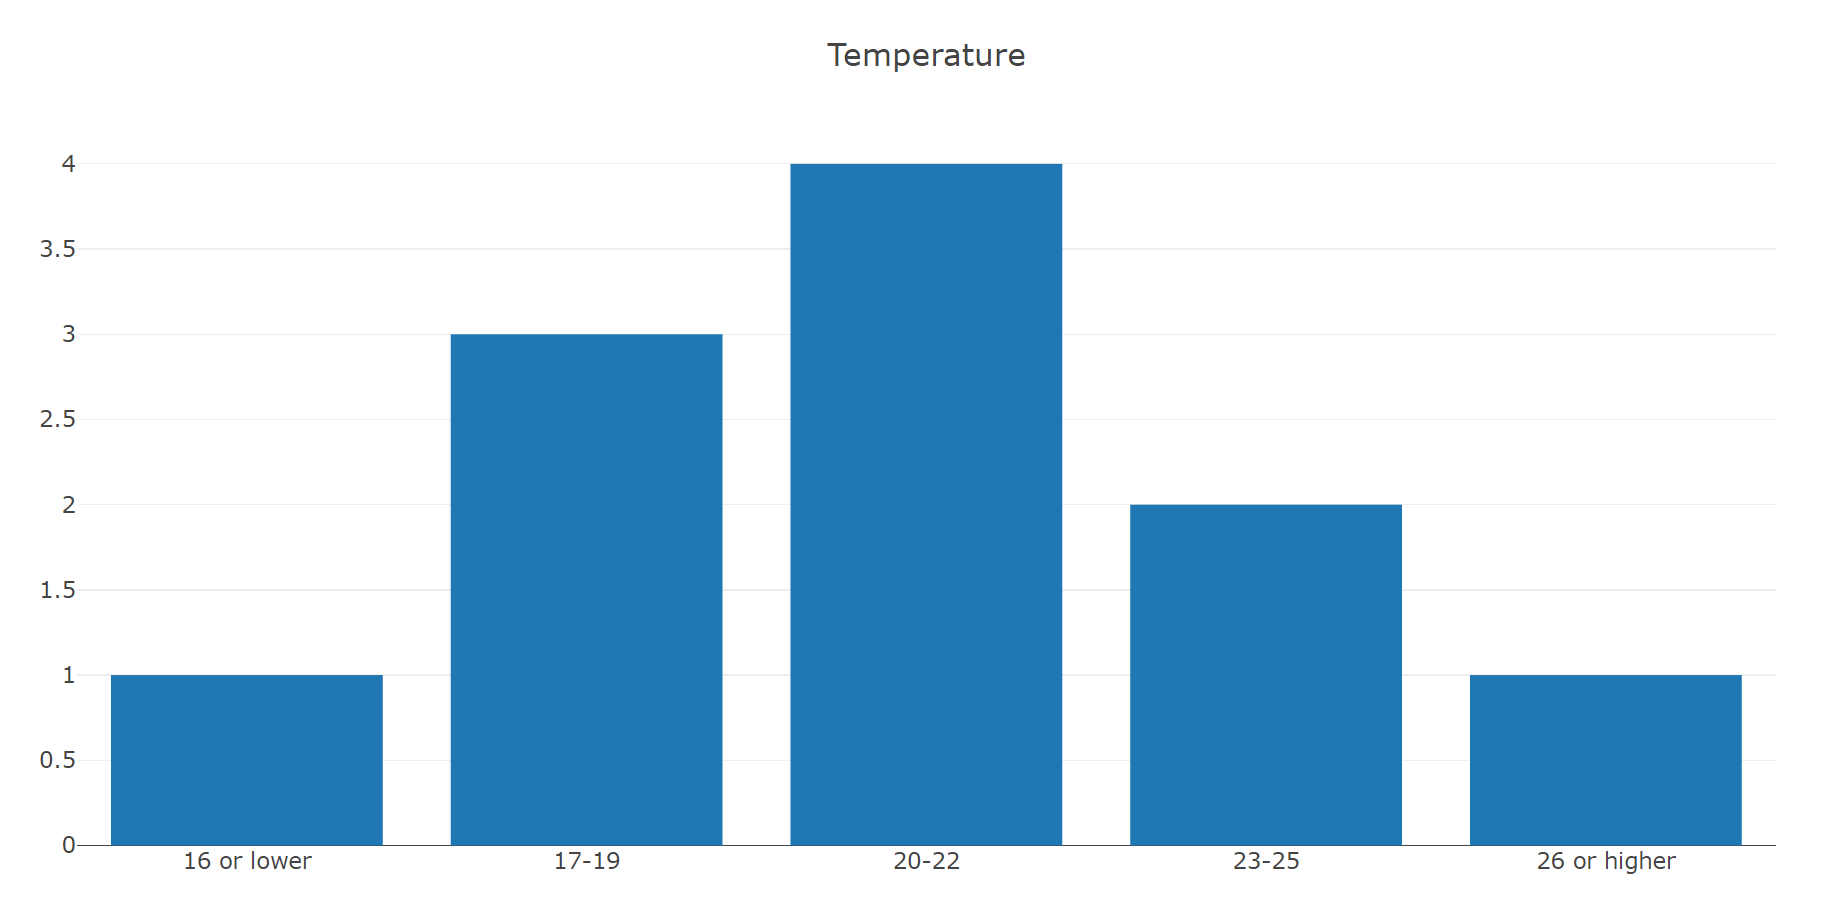
\includegraphics[scale=0.3]{exampleChart.png}
            \caption{Histogram temperatury}
        \end{figure}
        
        \subsection{Wybór platformy web-serwera}
	Aplikacja internetowa została stworzona za pomocą \textsl{frameworku} \texttt{Flask}. 
	\texttt{Flask} - \textsl{framework} do tworzenia aplikacji internetowych w języku \texttt{Python}, głównie do
	minimalistycznych aplikacji, które celowo zapewniają tylko podstawowe funkcje.
	
    \subsection{Generowanie wykresów w przeglądarce}
	Dla utworzenia wykresów w przeglądarce używana jest biblioteka \texttt{Plotly}, napisana w języku \texttt{JavaScript}.
	Biblioteka pozwala na utworzenie różnorodnych wykresów, z których dla danej aplikacji jest typem \textsl{bar}, odpowiadającym histogramowi. 
	Dane dla wykresów są przekazywane od serwera do przeglądarki jako odpowiedz na żądanie \texttt{HTTP}.

	Żądanie jest obsługiwane w języku \texttt{JavaScript} za pomocą ciągu funkcji, które zostały omówione w dalszej części dokumentacji.

    \subsection{Tworzenie wykresu}
    \begin{lstlisting}[frame=single, numbers=left, basicstyle=\ttfamily\small,
    caption={Funkcja do tworzenia histogramu za pomocą biblioteki \textsl{Plotly.js}}]
function drawChart(chart_divId, chart_title) {
  var trace = {
    type: 'bar',
    x: chartRanges[chart_title],
    y: chartData[chart_title],
  };

  var data = [ trace ];

  chart_title = chart_title.charAt(0).toUpperCase()+chart_title.slice(1);
  var layout = {
    title: chart_title,
    font: {size: 18}
  };

  Plotly.react(chart_divId, data, layout);
}
    \end{lstlisting}

    Dane z serwera są przekazywane w postaci tablicy. 
    Dodatkowym zadaniem skryptu w języku \texttt{JavaScript} jest kategoryzowanie danych
    dla różnych zakresów, zanim wykres będzie stworzony.

    Wartości dla osi \texttt{x} są nazwami zakresów, 
    do których może należeć wartość przekazana z serwera. 
    Dane zakresy są zdefiniowane statyczne i zadeklarowane na samym początku skryptu.
    \begin{lstlisting}[frame=single, numbers=left, basicstyle=\ttfamily\small,
caption={Zdefiniowany zakresy w skrypcie \texttt{JavaScript}}]
chartRanges = {
  "temperature" :
	     ["16 or lower", "17-19", "20-22", "23-25", "26 or higher"],
  "light": 
       ["349 or lower","350-450", "451-550", "551-650", "651 or higher"],
  "humidity":
	  ["0-20", "21-40", "41-60", "61-80", "81-100"]
}
    \end{lstlisting}

\subsection{Asynchroniczne wczytywanie danych z pliku}
    Dane, pobrane z czujników za pomocą platformy \textit{Raspberry Pi}, są przechowywane w pliku z rozszerzeniem \texttt{.csv}.
    Dla asynchronicznego wczytywania danych z pliku została użyty moduł \texttt{watchdog}.
    Dany moduł został użyty do monitorowania wybranych plików. 
    Wybór plików został zdefiniowany za pomocą wyrażeń regularnych. 
    Jeżeli dowolny plik o zadanym rozszerzeniu zostaje zmieniony, to serwer wysyła sygnał do przeglądarki,
    która została połączona z serwerem za pomocą gniazdek i nasłuchuje na te sygnały.
    Do obsługi różnego rodzaju sygnałów jest używany moduł \texttt{flask\_socketio}.
    \begin{lstlisting}[frame=single, numbers=left, basicstyle=\ttfamily\small, language=python,
    caption={Połączenie gniazdka na serwerze z gniazdkiem w przeglądrce}]
@socketio.on('connect')
def test_connect():
global thread
if thread is None:
  thread = socketio.start_background_task(target=background_thread)
    \end{lstlisting}

    Dla każdego sygnału mogą być zdefiniowane osobne funkcje. 
    W danej implementacji sygnał zostaje wysłany 
    jeżeli monitorowany plik został zmieniony, to serwer wysyła sygnał
    do przeglądarki za pomocą funkcji \texttt{on\_modified}, która dodatkowo
    wczytuje dane z pliku, żeby przekazać ich do przeglądarki.
   \begin{lstlisting}[frame=single, numbers=left, basicstyle=\ttfamily\small, language=python,
    caption={Definicja wątku, monitorującego zmiany w plikach o zadanych rozszerzeniu}]
def background_thread():
  global observer
  event_handler = CsvWatcher()
  observer = Observer()
  observer.schedule(event_handler, './', recursive=True)
  observer.start()
   \end{lstlisting}

\begin{lstlisting}[frame=single, numbers=left, basicstyle=\ttfamily\small, language=python,
    caption={Definicja funkcji wysyłającej sygnał i dane}]
def on_modified(self,event):
    global csvFileName
    data = readfile(csvFileName)
    socketio.emit('modified', {'data': data})
   \end{lstlisting}

    \subsection{Asynchroniczne odświeżanie wykresów w przeglądarce}
    Asynchroniczne odświeżanie wykresów umożliwia połączenie przeglądarki i serwera za pomocą gniazdek.
    Celem gniazdek jest asynchroniczna obsługa sygnałów, wysłanych z serwera.
    
    Do obsługi sygnału w języku \texttt{JavaScript} zostały zdefiniowane następujące funkcję:
\begin{lstlisting}[frame=single, numbers=left, basicstyle=\ttfamily\small,
    caption={Połączenie gniazdek w przeglądrce z serwerem i odebranie danych}]
var socket = io.connect('http://'+document.domain+':'+location.port);

socket.on('modified', function(data) {
    var newData = data['data'];
    start(newData)
});

\end{lstlisting}
\include*{telegram}
\include*{sensors}
\include*{auth}
\include*{raspbian}
\include*{summary}
\end{document}

